\documentclass[tikz,border=10pt]{standalone}
% Figure drawn in pixel-derived units: s = 0.014388 cm/px, centre (338,256) px
\usetikzlibrary{calc}
\begin{document}
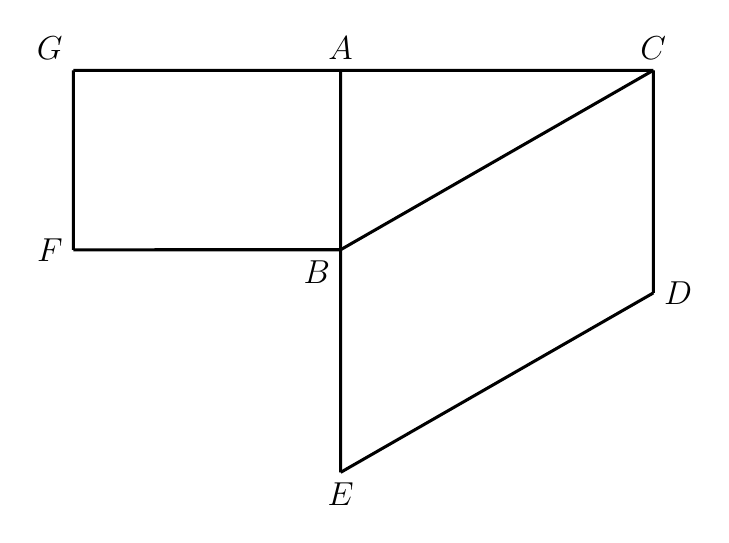
\begin{tikzpicture}[line width=1.1pt, line join=round, font=\fontsize{12}{14.4}\selectfont]
  % Points (converted from image pixels, y flipped)
  \coordinate (G) at (-3.6832161873003972,2.547919018408286);
  \coordinate (A) at (-0.28846778635545456,2.548563968951826);
  \coordinate (C) at (3.6827316809849684,2.549318436427016);
  \coordinate (F) at (-3.6827834699227884,0.2702767396118969);
  \coordinate (B) at (-0.2880350689778456,0.27092169015543677);
  \coordinate (D) at (3.683268790767166,-0.27780155364144066);
  \coordinate (E) at (-0.28749795919564797,-2.55619829991302);

  % Segments
  \draw (G) -- (C);   % top
  \draw (G) -- (F);   % left vertical
  \draw (C) -- (D);   % right vertical
  \draw (F) -- (B);   % horizontal at y=237
  \draw (A) -- (E);   % vertical x=318
  \draw (C) -- (B);   % diagonal C to B
  \draw (D) -- (E);   % diagonal D to E

  % Labels
  \node[above] at (A) {$A$};
  \node[above] at (C) {$C$};
  \node[above left] at (G) {$G$};
  \node[left] at (F) {$F$};
  \node[below left] at (B) {$B$};
  \node[right] at (D) {$D$};
  \node[below] at (E) {$E$};
\end{tikzpicture}
\end{document}